\subsection{Panoramica}
\begin{figure}[H]
\centering
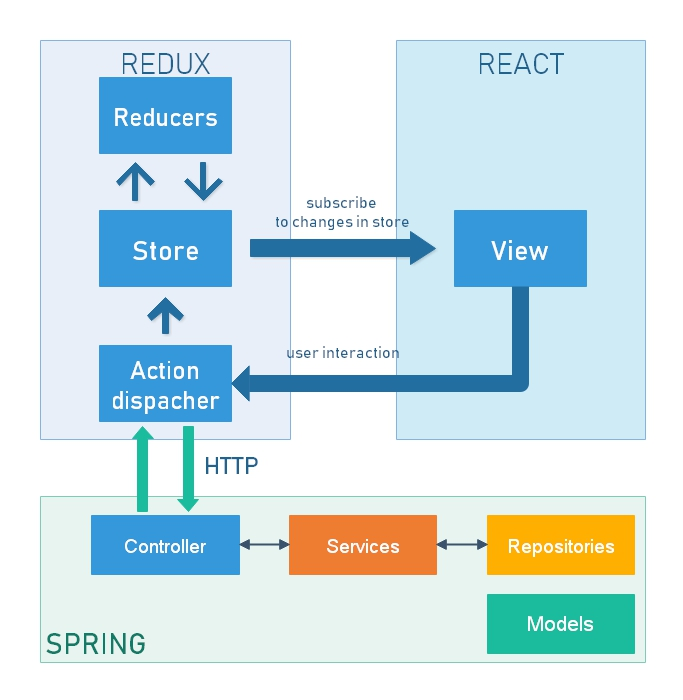
\includegraphics[width=17cm, keepaspectratio]{img/photo_2019-04-08_19-26-02.jpg} 
\caption{Exercise insert}
\end{figure}

\subsection{MongoDB Database}
\begin{figure}[H]
\centering
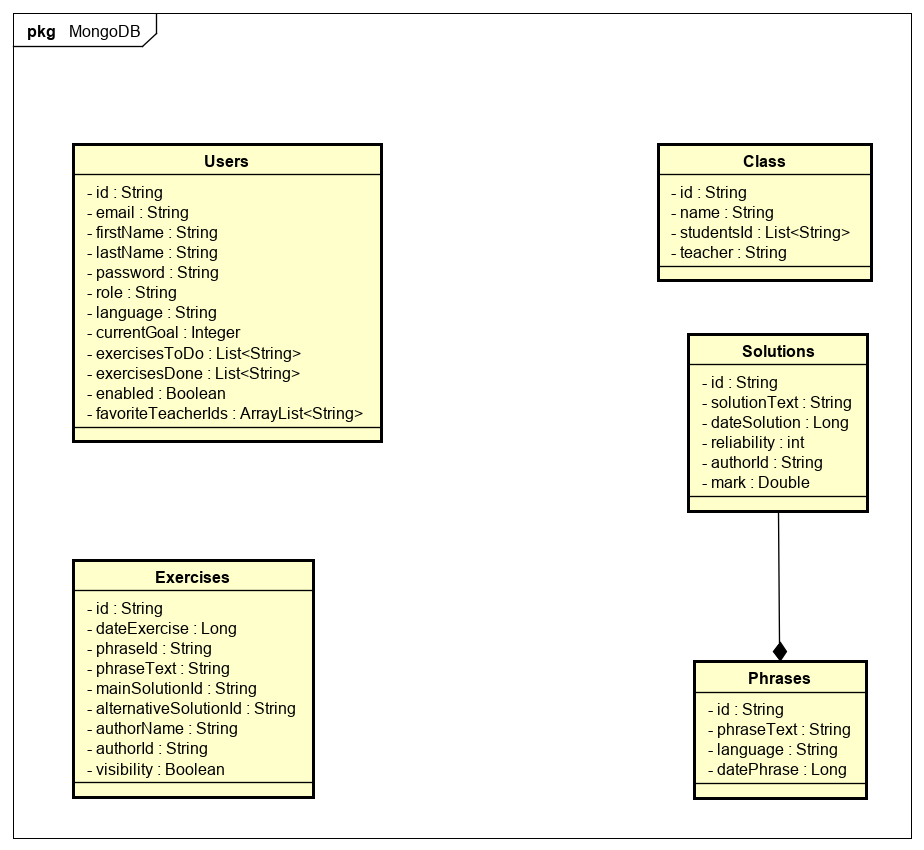
\includegraphics[width=17cm, keepaspectratio]{img/mongodb.png} 
\caption{MongoDB database}
\end{figure}
\newpage

\subsection{Design pattern utilizzati}
\subsubsection{Backend}
\paragraph{Adapter}\mbox{}\\

L'utilizzo della libreria di Freeling, per il pos-tagging, ha richiesto la creazione di un Adapter nella variante Object Adapter per poter adattare le funzionalità strettamente necessarie.
\begin{figure}[H]
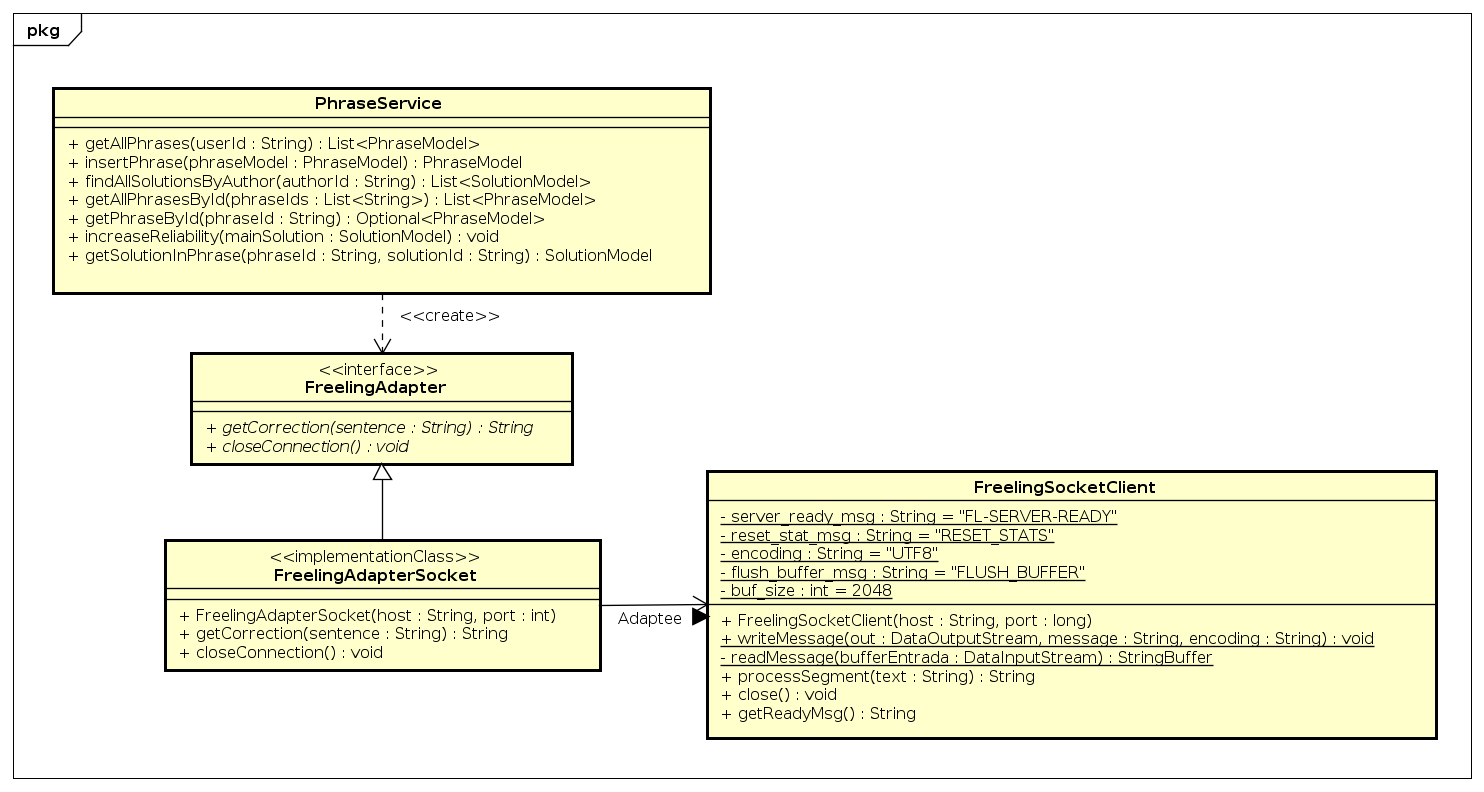
\includegraphics[width=17cm]{img/Adapter.png} 
\caption{Diagramma delle classi Adapter}
\end{figure}
La classe FreelingSocketClient viene fornita dai creatori della libreria e si occupa di realizzare la connessione con il server Freeling scritto in C++.
\paragraph{Controller - Service - Repository - Model}\mbox{}\\

L'architettura realizzata all'interno di Spring Web consta nella presenza di:
\begin{itemize}
\item \textbf{Controller}: a cui viene delegato il compito di gestire le richieste provenienti dalla parte frontend e la cattura delle eccezioni;
\item \textbf{Service}: realizzano la business-logic;
\item \textbf{Repository}: realizzano il layer di persistenza gestendo la base di dati;
\item \textbf{Model}: rappresentano oggetti  Plain Old Java Object, un'istanza di un model rappresenta un documento di una collezione.
\end{itemize}
\begin{figure}[H]
\centering
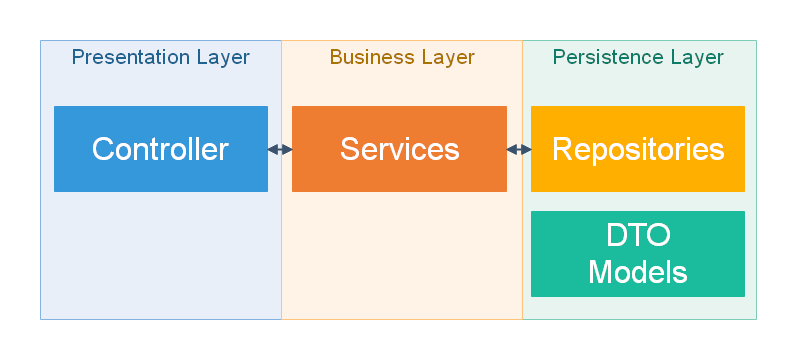
\includegraphics[width=14cm]{img/springArch.png}
\caption{Scherma generale architettura in Spring}
\end{figure}

\subsubsection{Frontend}
\paragraph{Redux}\mbox{}\\

\begin{figure}[H]
    \centering
	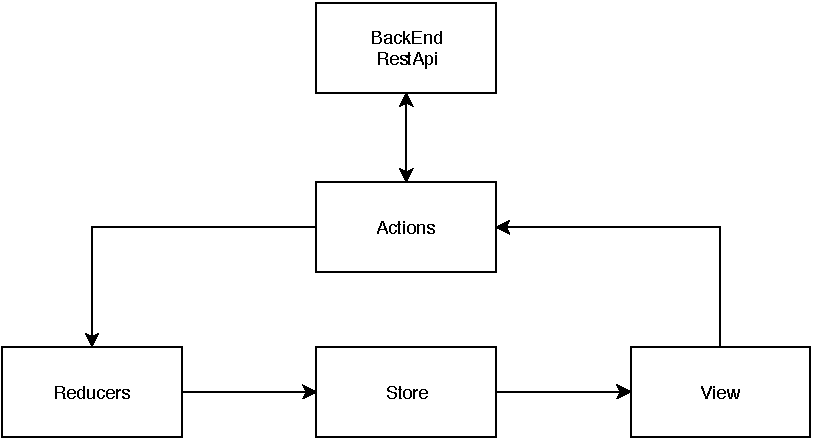
\includegraphics[width=0.7\linewidth]{img/Flux.pdf}
	\caption{Schema del design pattern Flux}
\end{figure}

Per la frontend viene utilizzato React con design pattern Redux, un'evoluzione del design pattern Flux.
In Redux, tutti i dati scorrono in modo unidirezionale attraverso i seguenti componenti:
\begin{itemize}
    \item \textbf{Store: }oggetto immutabile che contiene l'intero stato dell'applicazione in maniera centralizzata;
    \item \textbf{Reducers: }sono funzioni pure. Ogni volta che i Reducer ricevono una nuova azione, 
    processano l'azione ricevuta e, in caso sia necessario apportare delle modifiche allo stato, restituiscono un nuovo oggetto 
    \item \textbf{Action creators: }funzioni che facilitano la gestione del dispatch (creazione di azioni da mandare ai reducers); 
    \item \textbf{View: }componenti grafiche, il loro contenuto dipende dallo store. Sono implementate attraverso un \textit{Observer Pattern} sullo store stesso.
    Ad ogni cambiamento di stato prodotto da un reducers vengono renderizzate le componenti collegate ad esso.
\end{itemize} 


\subsection{Diagrammi dei package}
\subsubsection{Data Transfer Object}
Le classi Helper rappresentano Data Transfer Object (DTO), vengono utilizzate dalla classe \texttt{Controller.java} per fornire un oggetto per il trasferimento dati dalla frontend senza ricorrere a JSON troppo complessi.

\subsubsection{Builder}
I model sono dotati ognuno di un builder, tale classe interna non è codificata ma realizzata tramite un plugin denominato lombok. A seguire viene mostrato un esempio di un builder creato automaticamente.
\begin{figure}[H]
\centering
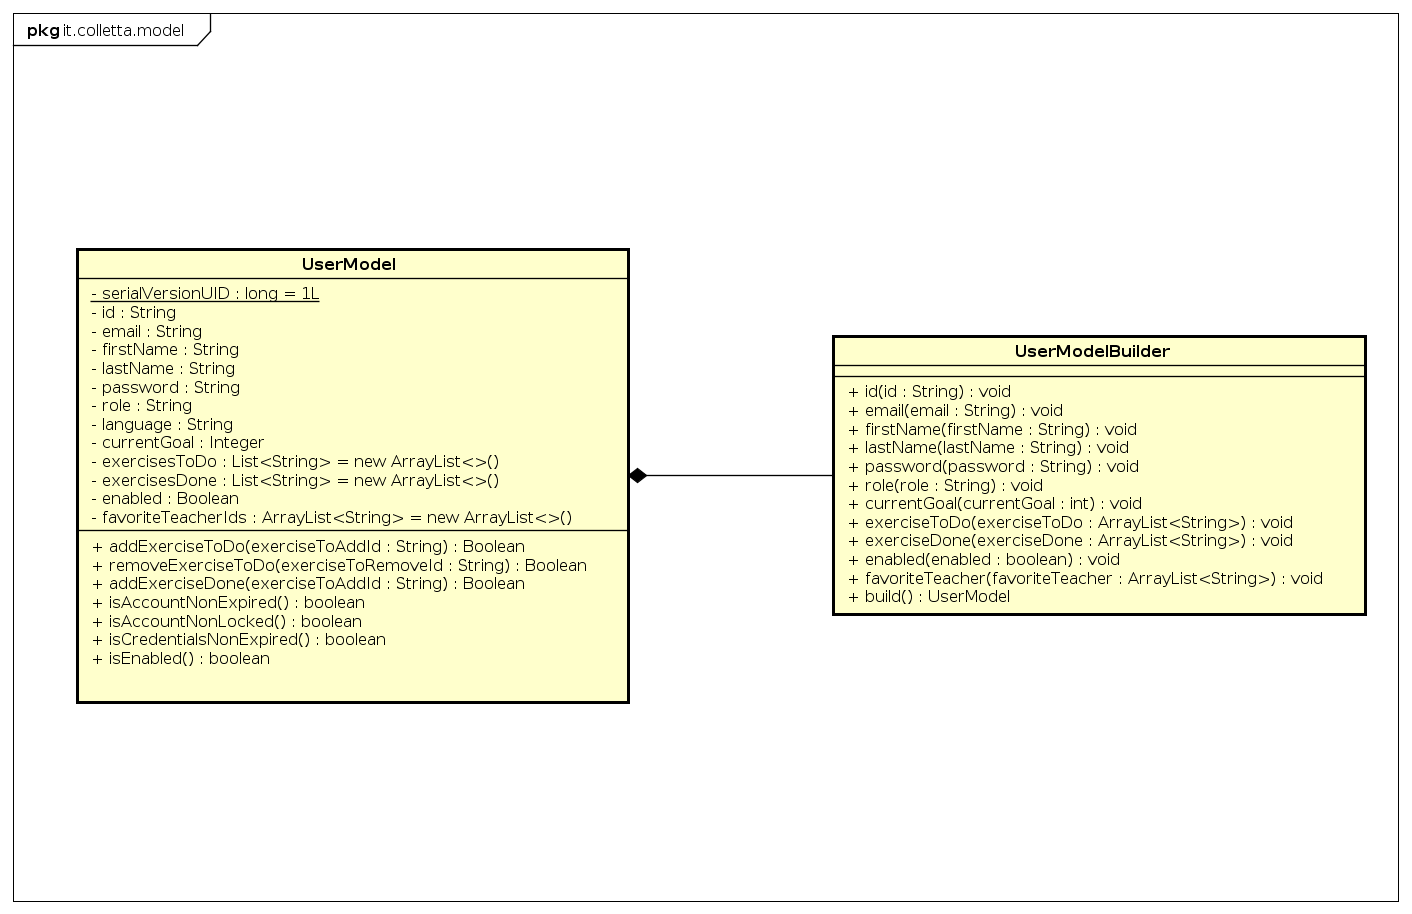
\includegraphics[width=15cm]{img/builder.png}
\caption{Esempio di builder presente nella classe UserModel}
\end{figure}

\subsection{Model}
Viene di seguito riportato il diagramma delle classi del package model.
\begin{figure}[H]
\centering
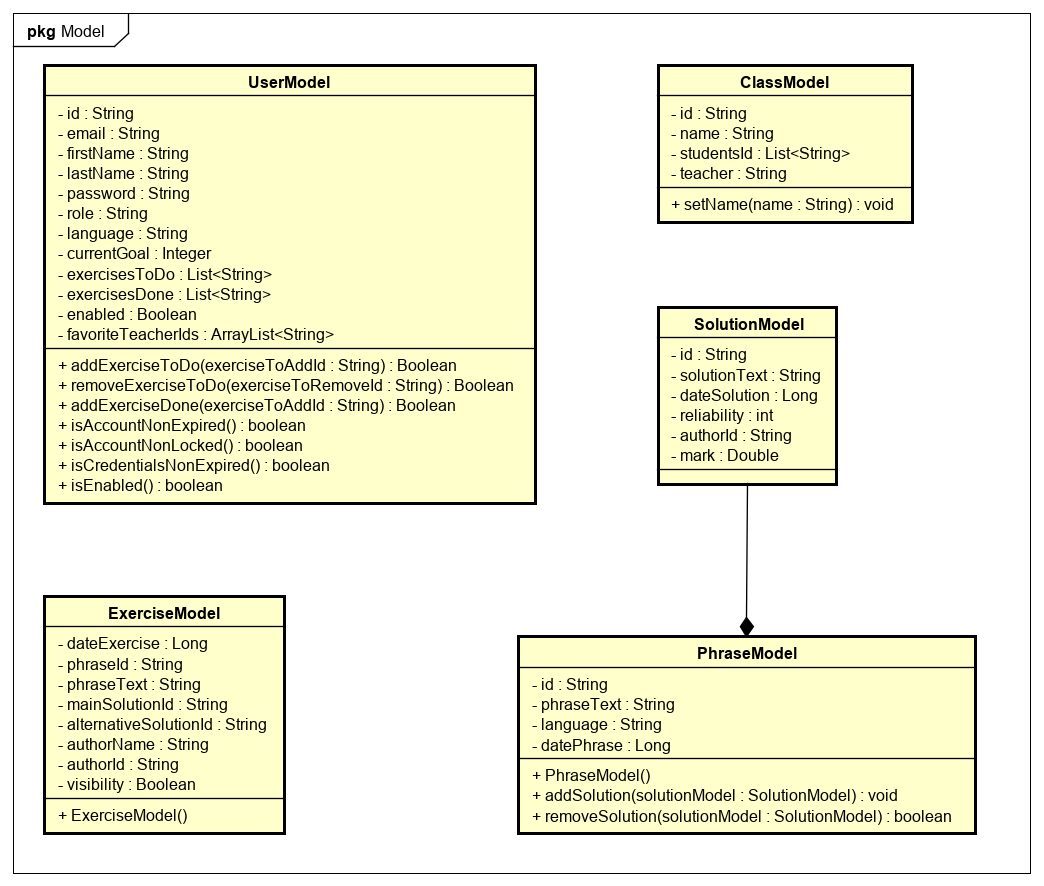
\includegraphics[width=17cm, keepaspectratio]{img/model.png} 
\caption{Model}
\end{figure}
\newpage

\subsection{Controller e service}
Viene di seguito riportato il diagramma delle classi di package controller e service.
\begin{figure}[H]
\centering
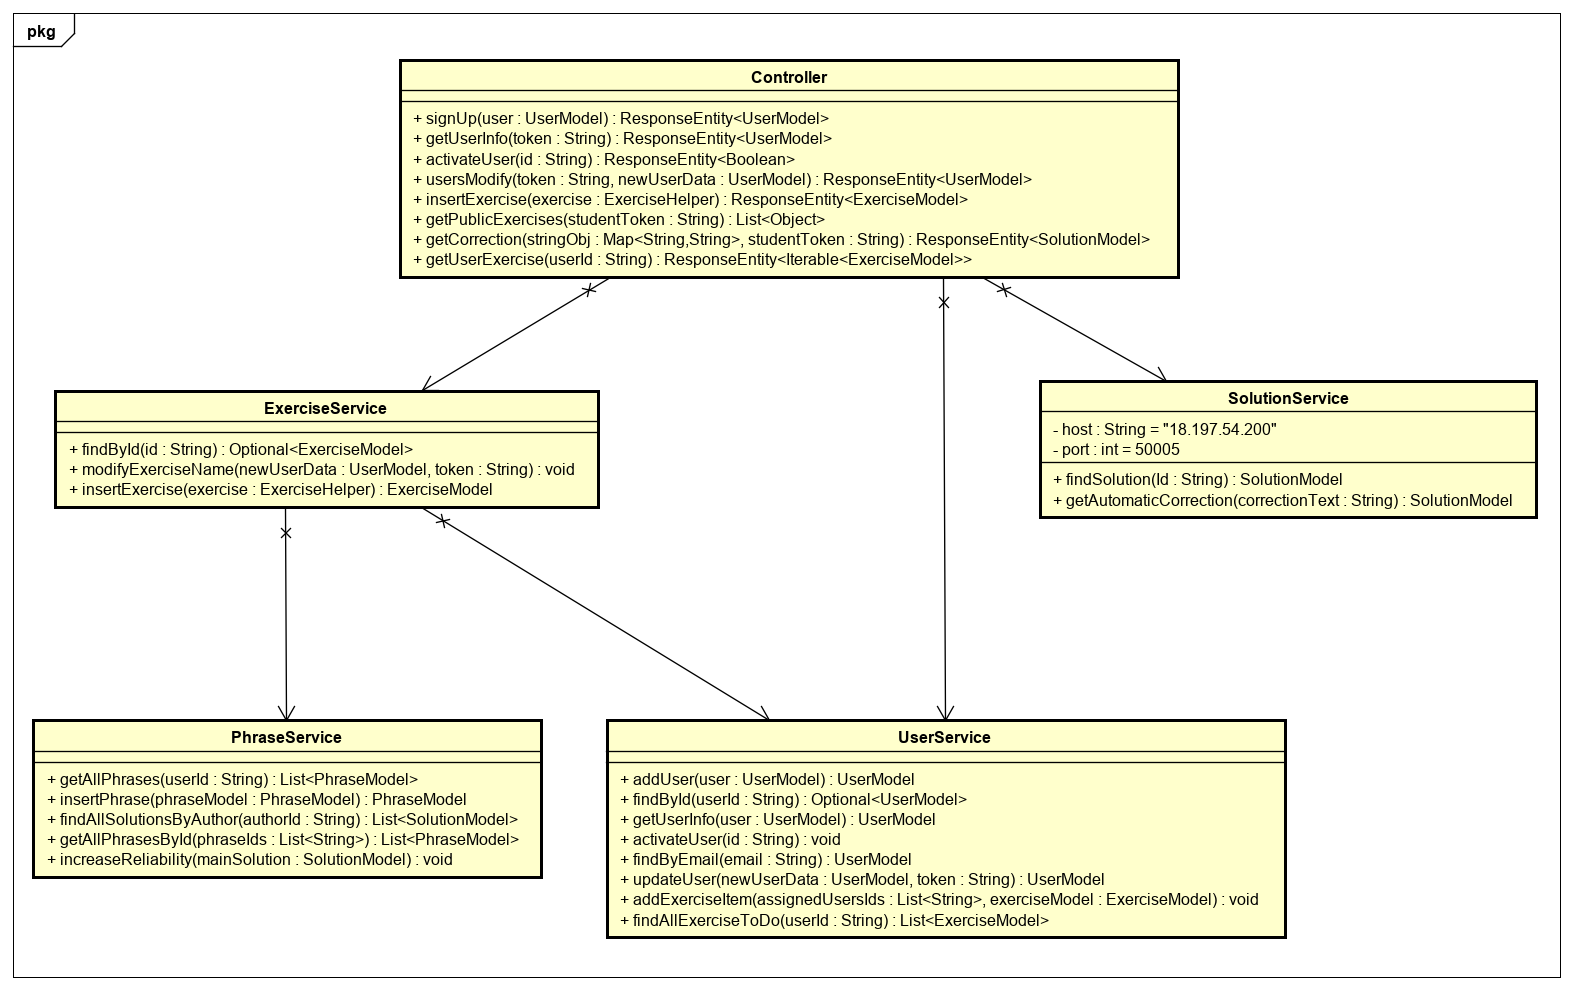
\includegraphics[width=17cm, keepaspectratio]{img/Controller-service.png} 
\caption{Controller e Service}
\end{figure}
\newpage
\subsection{Service e repository}
Viene di seguito riportato il diagramma delle classi di package service e repository.
\begin{figure}[H]
\centering
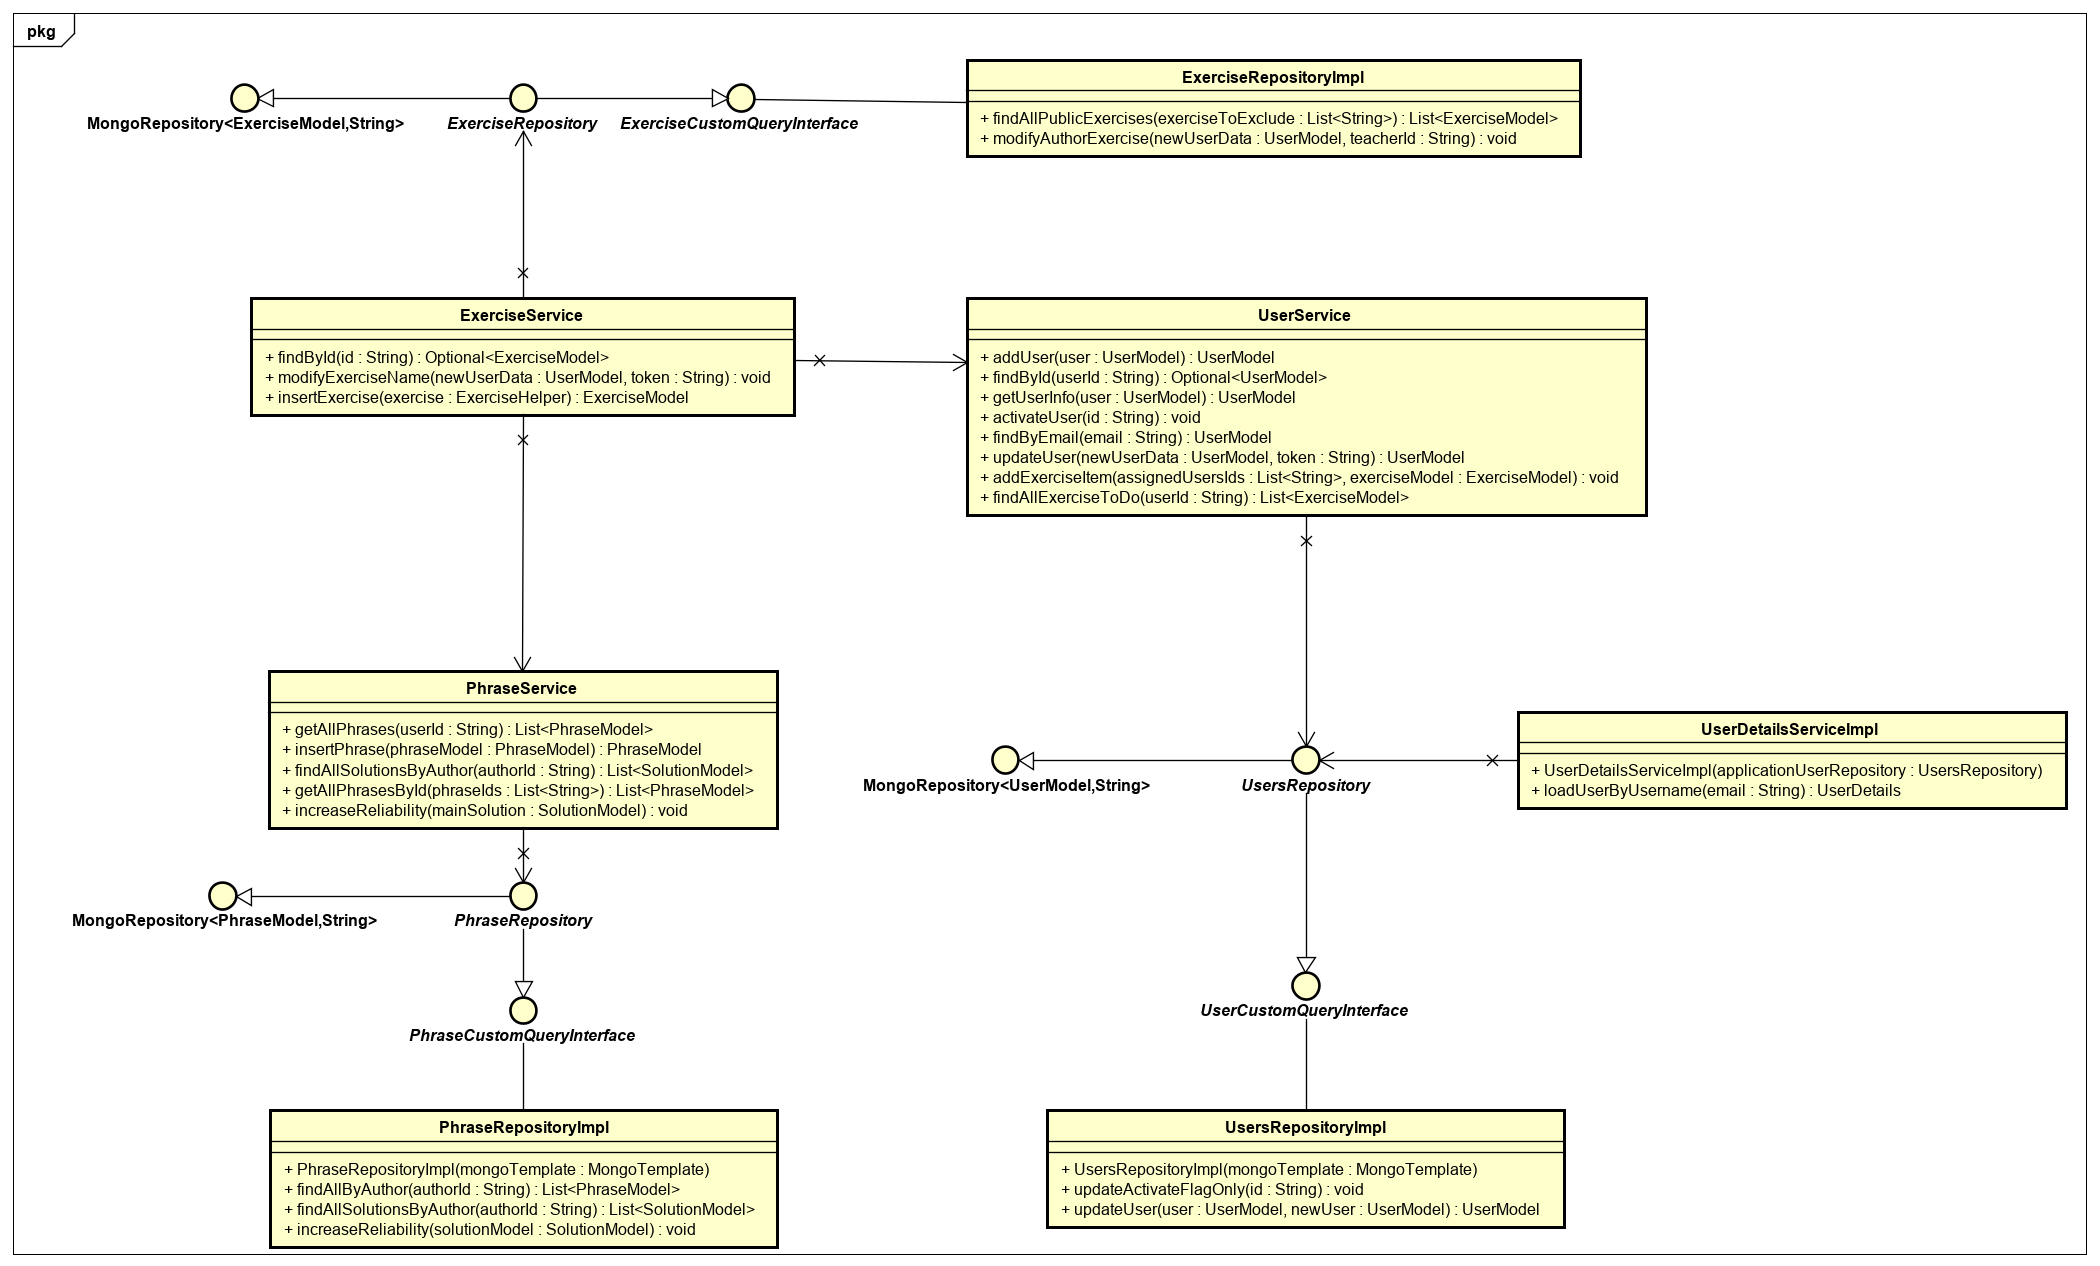
\includegraphics[width=17cm, keepaspectratio]{img/Service-repository.png} 
\caption{Service e Repository}
\end{figure}
\newpage
\subsection{Diagrammi di sequenza}
\subsubsection{Inserimento di un utente}
Il diagramma di sequenza rappresenta l'azione di inserimento di un esercizio nel sistema
\begin{figure}[H]
\centering
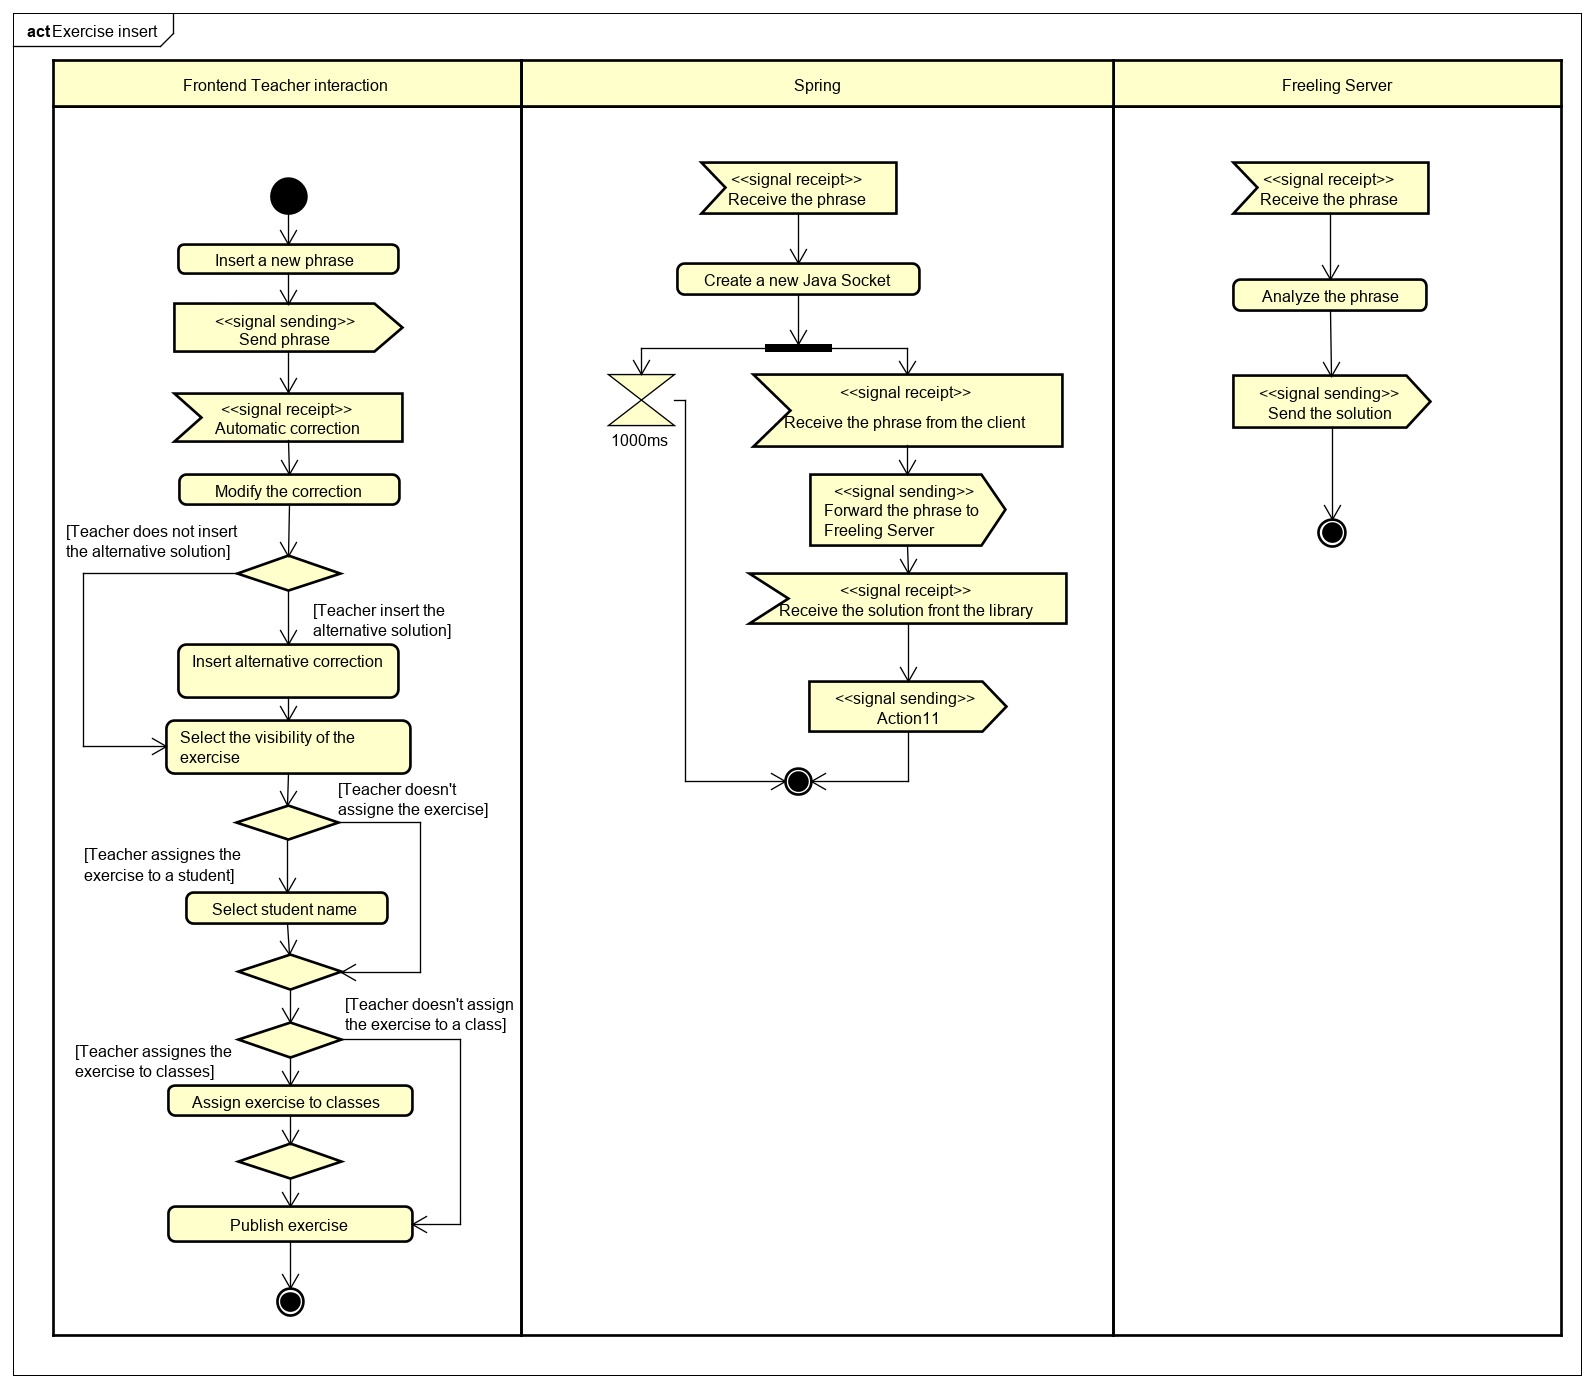
\includegraphics[width=17cm, keepaspectratio]{img/Exercise-insert.png} 
\caption{Exercise insert}
\end{figure}

\begin{figure}[H]
\centering
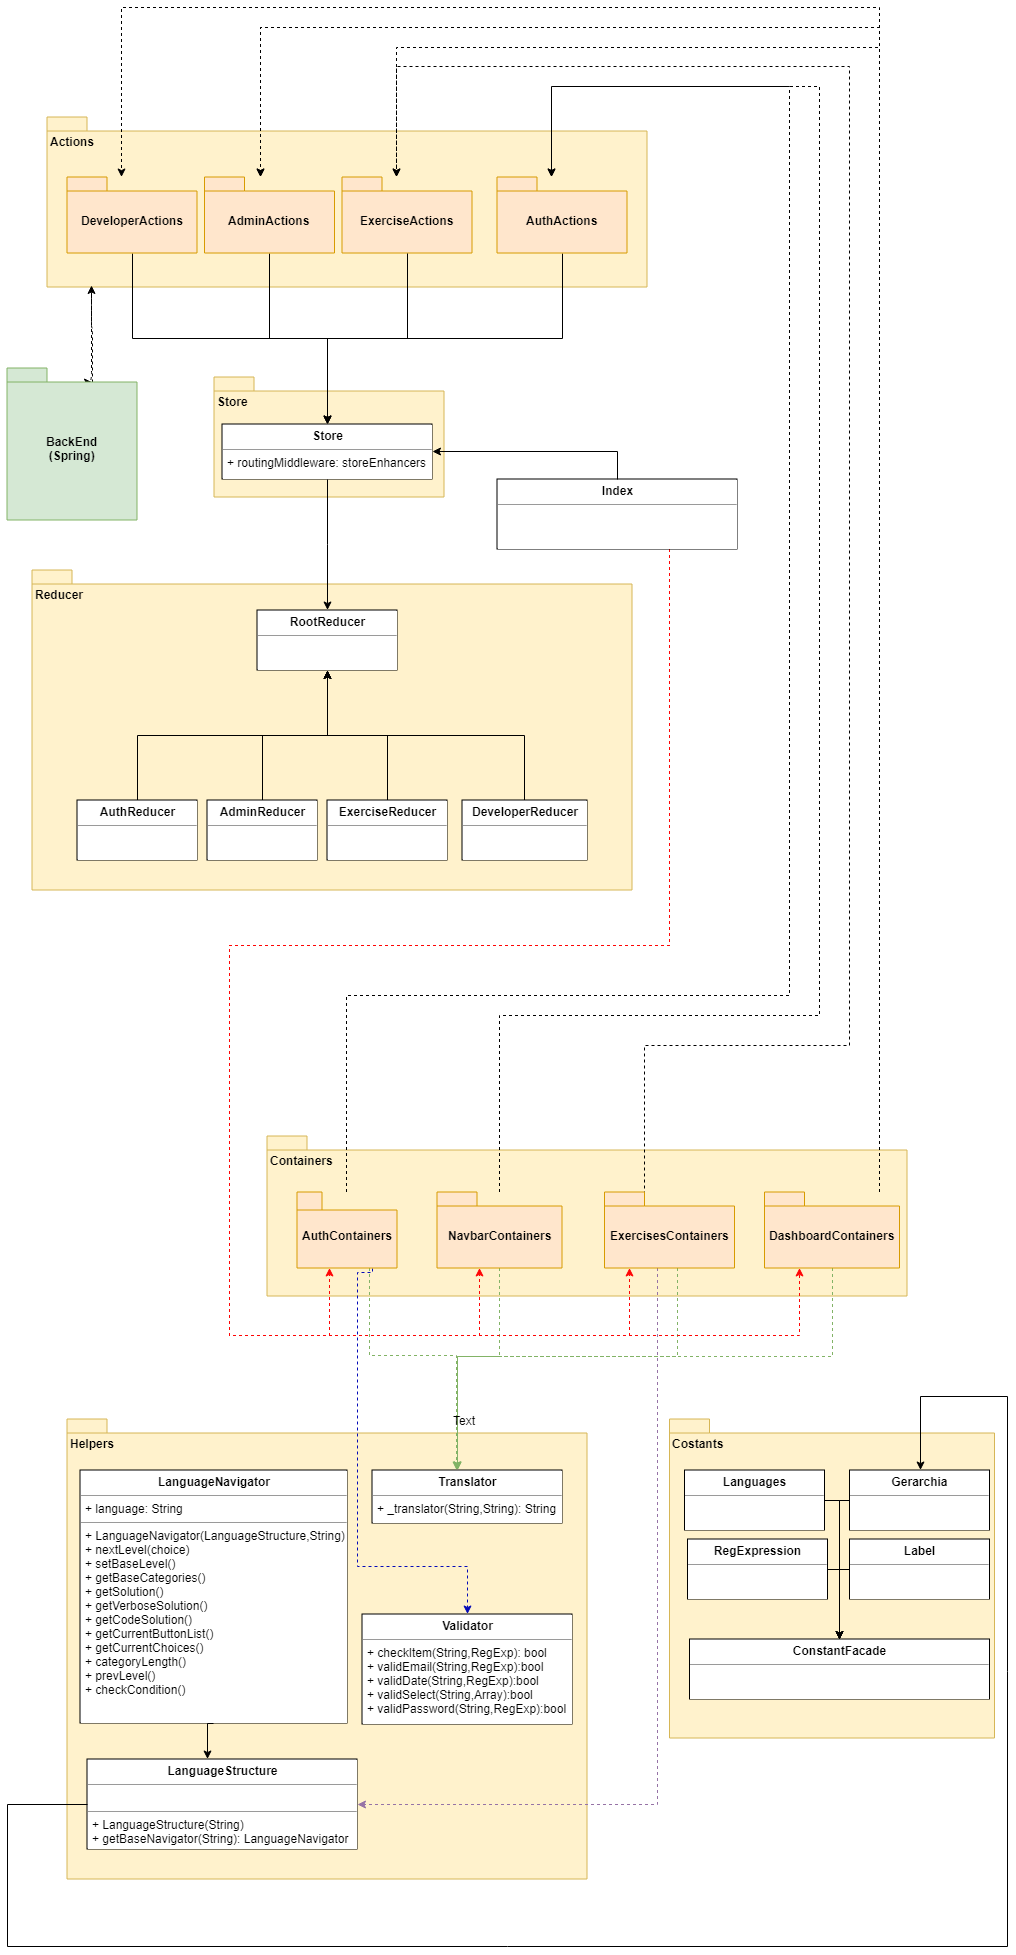
\includegraphics[width=18cm, height=23cm]{img/ReactSpec1.png} 
\caption{UML - FrontEnd}
\end{figure}

\subsubsection{Login}
Il diagramma di sequenza riportato qui di seguito raffigura il processo di login, durante il quale l'utente che vuole accedere può essere autenticato dal sistema.
\begin{figure}[H]
\centering
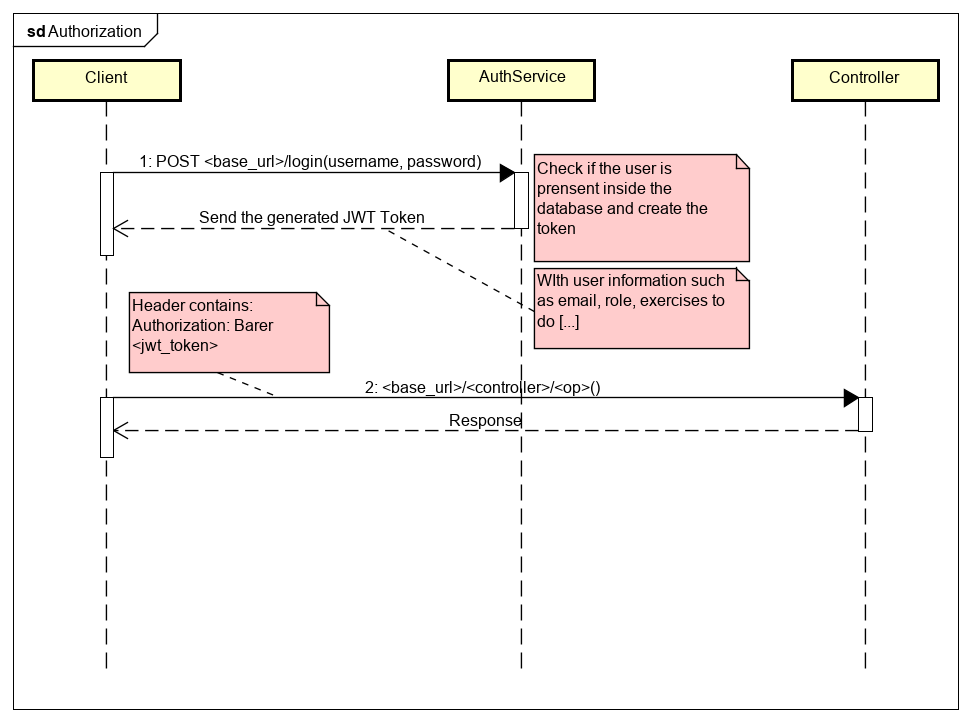
\includegraphics[width=17cm, keepaspectratio]{img/Authorization.png} 
\caption{Authorization}
\end{figure}




